\begin{abstract}
Cumacea crustaceans serve as vital indicators of benthic health in marine ecosystems. This study investigates the influence of environmental parameters on their genetic makeup in the North Atlantic, focusing on Icelandic waters. We analyze mitochondrial 16S rRNA gene sequences from 62 Cumacea specimens collected across varying depths. We use \textit{aPhyloGeo} software to correlate these sequences with environmental data encompassing temperature ($^\circ$C) (see Figure \ref{fig:fig1}e), oxygen concentration (mg/L) (see Figure \ref{fig:fig1}f), depth (m) (see Figure \ref{fig:fig1}c), and other relevant factors.

Our analyses reveal significant spatial variation in environmental parameters, particularly depth (m), and temperature ($^\circ$C) (see Figures \ref{fig:fig1}c and \ref{fig:fig1}e). Cumacean diversity also varied across habitat types (see Figure \ref{fig:fig4}). Interestingly, specific genetic sequences correlated with wind speed and oxygen levels (see Figures \ref{fig:fig5} and \ref{fig:fig6}), suggesting potential local adaptations to these fluctuating environmental conditions.

These initial findings highlight the need for further exploration to understand the relationships between Cumacean genetics and their environment. This study lays the groundwork for establishing correlations between specific mitochondrial gene regions and environmental variables. If substantiated, these findings would support the hypothesis of natural selection driving local adaptation of Cumacea to environmental gradients in the face of climate change. The \textit{aPhyloGeo} Python package is freely and publicly available on \href{https://github.com/tahiri-lab/aPhyloGeo}{GitHub}, and it is also available on \href{https://pypi.org/project/aphylogeo/}{PyPi}, to facilitate complex analyses.

\end{abstract}

\section{Introduction}\label{introduction}
The vast North Atlantic and subarctic regions, particularly the Icelandic area and its surrounding waters, present significant ecological interest \citep{schnurr_composition_2014, uhlir_adding_2021}. The seas around Iceland exhibit a remarkable diversity of water bodies originating from various sources \citep{brix_iceage_2014}. These unique oceanographic and hydrographic characteristics shape {benthic habitats}\footnote{Benthic habitats are areas on the bottom of the ocean or lake, including the sediments and organisms that live there \citep{levin2009ecological}.} through multiple parameters such as depth gradients, water mass indicators, and specific habitat configurations \citep{meisner_benthic_2014, uhlir_adding_2021}. Consequently, research in these areas enhances our understanding of deep-sea ecosystems and the patterns of biodiversity within them \citep{rogers2007corals, meisner_prefacebiodiversity_2018}.

The biological and environmental baseline data collected by the IceAGE project and its predecessors BIOFAR and BIOICE, which studied the biodiversity of the Faroe Islands and Iceland, are invaluable resources for addressing two significant issues facing present and future generations: the impacts of climate change and seabed mining. For decades, the North Atlantic region around Iceland has been recognized as a crucial area for regulating global {thermohaline circulation}\footnote{This is a system of ocean currents produced by differences in seawater density, which in turn are determined by temperature (thermo) and salinity (haline) \citep{talley2013closure}.} \citep{meisner_prefacebiodiversity_2018}. The Greenland, Iceland, and Norwegian (GIN) seas, along with the high-latitude North Atlantic, play a crucial role in modern deep-sea ventilation. These surface waters are critical for global deep-sea renewal and vital to the thermohaline circulation \citep{johannessen_relationship_1994}. One of the most significant changes observed is the formation of cold, deep water. With the loss of Arctic sea ice, this process has slowed, likely impacting the dynamics and chemistry in the regions studied during the IceAGE expedition \citep{meisner_prefacebiodiversity_2018}.

There is a growing international interest in deep-sea resource extraction \citep{mengerink_call_2014}, particularly targeting mid-ocean ridges and other active geothermal areas. The ridges around Iceland, such as the Reykjanes Ridge, are home to hydrothermal vent sites. Assessing the extent of damage and loss of ecosystem services caused by climate change and mining activities is challenging without robust baseline data \citep{meisner_prefacebiodiversity_2018}.

Crustaceans of the taxon Peracarida Calman, 1904, often constitute a significant portion of macrobenthic communities in Arctic and subarctic waters. They are widely dispersed across the continental shelf and slope of northern seas. This study focuses on the peracarid taxon Cumacea Krøyer, 1846, which plays a crucial role as an indicator of the health of marine ecosystems due to their high susceptibility to environmental fluctuations \citep{stransky_diversity_2010}. Thus, their diversity and abundance are likely to represent the quality of local environments, which makes them crucial for ecological monitoring studies \citep{hessler1967faunal}. Cumaceas are also part of the food web of benthic ecosystems, providing prey for numerous species of fish and marine invertebrates \citep{rehm2009cumacea}. These organisms are primarily bottom-dwelling marine benthic crustaceans, spending much of their lives buried in or near sediments. Consequently, they are presumed to have limited dispersal abilities and are unlikely to move great distances \citep{uhlir_adding_2021}.

Unlike the benthic invertebrates inhabiting the rocky intertidal environments of the Northwest and Northeast Atlantic, the evolutionary history and dynamics of deep-sea benthic invertebrates in the North Atlantic are less understood \citep{jennings_phylogeographic_2014}. Although many studies reveal intriguing patterns of genetic distribution among deep-sea benthic invertebrates (e.g., \citep{wilson_historical_1998, havermans_genetic_2013}), understanding the origin and demography of deep Atlantic biota is fundamental for comprehending their relationship with ongoing climate change, which should be considered a factor in the range expansion of deep-sea fauna \citep{jennings_phylogeographic_2014}.

In response to the current climate emergency, this study aims to undertake an in-depth analysis of the influence of extreme climatic parameters and environmental peculiarities on Cumacea (crustaceans: Peracarida). Specifically, we seek to determine whether there is a correlation between the genetic information of the mitochondrial 16S rRNA gene region of Cumacea species sampled and the characteristics of their habitats. If applicable, we'll determine which of our environmental attributes correlates best with a specific genetic sequence (i.e. window) and identify the protein associated with that gene. Our approach includes a comparative study to validate different phylogeographic models by comparing them with environmental factors found inside and outside the waters of the North Atlantic seas around Iceland. Phylogeographic models are computational tools that analyze the relationships between the genetic structures of populations and their geographical distributions. By incorporating environmental variables, we can interpret how the latter impacts the genetic distribution of Cumacea species. Additionally, we will update a Python package (currently in beta), called \textit{aPhyloGeo}, to simplify these complex analyses.

This paper is organized as follows: Section \autoref{related-works} reviews related work on the biodiversity and biogeography of deep-sea benthic invertebrates. Section \autoref{materials-methods} details the materials and methods used in this study, including sampling procedures, genetic analyses, and environmental data collection. Section \autoref{metrics} discusses the metrics used to evaluate phylogeographic models and the impact of environmental factors. Section \autoref{results} presents the results of our analyses. Finally, Section \autoref{conclusion} summarizes our findings and discusses their implications for future research and conservation efforts.

\section{Related Works}\label{related-works}
Many studies have investigated the relationship between genetics and the climatic conditions of various regions. These studies have shown how organisms adapt to their environment \citep{fc_genomic_2012} and helped develop conservation plans to maintain biodiversity and protect endangered species \citep{balkenhol_identifying_2009}.

\cite{koshkarov_phylogeography_2022} proposed a phylogeographic approach based on an algorithm called \textit{aPhyloGeo} to study the correlation between severe acute respiratory syndrome coronavirus 2 (SARS-CoV-2) variants and their geographical characteristics. More recently, \cite{li_aphylogeo-covid_2023} developed an interactive platform called \textit{aPhyloGeo-Covid} to facilitate these analyses. We elaborate on the extension of the \textit{aPhyloGeo} software and its use in this study later in this article.

The correlation between genetics and environmental parameters has been confirmed in studies of various organisms, supporting the influence of habitat characteristics on genetic diversity \citep{colosimo_widespread_2005,cheviron_genomic_2012}. \cite{ghalambor_adaptive_2007} have demonstrated that environmental characteristics, such as water temperature, can affect the genetics of guppy populations (\emph{Poecilia reticulata}) by shaping their phenotypic plasticity and promoting rapid genetic adaptation. \cite{cheviron_genomic_2012} also concluded that there is a correlation between vertebrate genetics and habitat properties, particularly in high altitudes. Study on Threespine Sticklebacks (\emph{Gasterosteus aculeatus}) by \citep{colosimo_widespread_2005} support this correlation, implying that species acclimatization to climate change results from the interaction between genetic variation among populations and selection pressures caused by environmental changes \citep{hoffmann_climate_2011}.

However, studies have highlighted the complexity of the relationships between genetics and the environment, influenced by factors such as genotype-environment interaction and natural selection, making it challenging to identify clear causal relationships \citep{balkenhol_identifying_2009}. Distinguishing between the direct and indirect effects of the environment on genetics can be just as complex  \citep{manel_perspectives_2010, balkenhol_landscape_2019}. The methods available to measure genetic and environmental characteristics and logistical constraints often limit the scale of studies \citep{manel_perspectives_2010, shafer_widespread_2013}. This can explain why research into Cumacea’s environment and genetics has been little explored, even though they remain essential for understanding how these deep-sea invertebrates adapt to fluctuating environmental conditions.

As stipulated in the hypothesis of Darwin, individuals best adapted to their environment are likely to survive, reproduce, and evolve. The objective of this study is to deepen and strengthen the natural selection hypothesis by examining whether there are one or more locations within the DNA sequence of Cumacea, specifically in the mitochondrial 16S rRNA gene, that could correlate not only the segments of the sequence (i.e., windows) but also the Cumacea to a specific property of their environment. 

We are reporting crucial information on the genetic diversity of Cumacea in the face of environmental fluctuations, to further our knowledge of how marine species adapt to climatic variations. This is essential for predicting and regulating the impact of climate change on marine biodiversity. This study initiates further research on other species and in different geographical regions. By extending the research and analysis to various environments and taxonomic groups, scientists will gain a broader picture of the adaptation and resilience of marine biodiversity to climate change. We report essential information on the genetic diversity of Cumacea in the face of environmental fluctuations, to further our knowledge of how marine species adapt to climatic variations. This information is essential for predicting and managing the impact of climate change on marine biodiversity. This genetic and environmental information will highlight critical habitats and regions of high conservation interest. Regions showing high genetic fluctuation or areas vulnerable to environmental variation can be put forward for conservation efforts and the establishment of marine protected areas. This study initiates further research on other species and in different geographical regions. By extending the research and analysis to various environments and taxonomic groups, scientists will gain a broader picture of the adaptation and resilience of marine biodiversity to climate change.

\section{Our Contribution}

Our study investigates the genetic variation of Cumacea populations concerning environmental factors. We aim to identify genetic regions with high mutation rates and their correlation with geographical distribution patterns. Through robust analytical methods, including dissimilarity calculations and phylogenetic reconstruction, we provide insights into the genetic adaptation of marine crustaceans. Our findings contribute to understanding evolutionary dynamics in marine ecosystems.

\section{Materials and Methods}\label{materials-methods}
In this section, we will describe our data, followed by an outline of the main steps used in data preprocessing and the software \textit{aPhyloGeo}. 

\subsection{Description of the data}
The study area is located in a northern region of the North Atlantic, including the Icelandic Sea, the Denmark Strait, and the Norwegian Sea. The specimens examined in this study were gathered during the IceAGE project (Icelandic marine Animals: Genetic and Ecology; Cruise ship M85/3 in 2011; \cite{brix_iceage_2014}), which investigated the deep continental slopes and abyssal waters around Iceland \citep{meisner_prefacebiodiversity_2018}. The sampling period for the specimens included in this study was from August 30 to September 22, 2011, and they were collected at depths ranging from 316 to 2568 m.  Information about the sampling plan, sample processing, the steps of DNA extraction, PCR amplification, sequencing, and the extracted and aligned DNA sequences are available in the article by \citep{uhlir_adding_2021}.

\subsection{Data pre-processing}
We used data from the IceAGE project and related data from the BOLD Systems database, both of which are accessible through the article by \citep{uhlir_adding_2021}. Given the enormous scope of attributes in these databases, we selectively reduced the number of attributes and samples. 

1.    Specifically, we omitted attributes that were not relevant to the context of this study, were entirely or nearly invariable (non-numerical data), or had abundant missing data (>95\%). 

From the IceAGE project dataset, we considered 62 specimens out of the 495 available.

2.    Subsequently, we calculated the variance for each of the selected numeric attributes to eliminate those with zero or low variance (cut-off ≤ 0.1). Equation \ref{variance} provides the formula for variance used in this study.

\begin{equation}\label{variance}
    S^2 = \frac{\sum_{i=1}^{n} (x_i - \bar{x})^2}{n-1}
\end{equation}

where $S^2$ is the sample variance, $x_i$ represents each value in the dataset, $\bar{x}$ the average of all values in the dataset, and $n$ the number of values in the dataset.

Only salinity was removed from the previously selected numerical attributes ($S^2 = 0.02146629$). This selection of attributes and data resulted in a data table containing 62 rows ($n=62$) and 18 columns (number of attributes). 

From the IceAGE database, 14 attributes were selected. These consist of the geographical coordinates such as: 

\begin{itemize}
\item The latitude (decimal) and longitude (decimal) taken at the beginning (see           Figures \ref{fig:fig1}a and \ref{fig:fig1}b) and at the end of sampling. The         increase in latitude, in particular, has been highlighted by several studies         as being linked to the decline of marine biodiversity on a global scale              \citep{lambshead_latitudinal_2000, gage_diversity_2004}. 

\item These geographic data are divided into five sectors across the seas around           Iceland: the Denmark Strait ($n=28$), the Iceland Basin ($n=15$), the Irminger       Basin ($n=12$), the Norwegian Sea ($n=4$), and the Norwegian Basin ($n=3$). 
\end{itemize}

Concerning the environmental attributes in this database, we included:
\begin{itemize}
\item The depth (m) at the beginning (see Figure \ref{fig:fig1}c) and end of               sampling as well as the temperature ($^\circ$C) (see Figure \ref{fig:fig1}e)         and oxygen concentration (mg/L) (see Figure \ref{fig:fig1}f) of the water            depending on the depth at which the specimens were sampled. These properties         of water bodies are drivers of deep-sea biodiversity and biogeography, with          oxygen being a limiting factor for living organisms                                  \citep{keeling_ocean_2010}. In addition to these contributions, the increase         in depth \citep{rex_global_2006,costello_marine_2017} and the decrease in            water temperature at depth \citep{lambshead_latitudinal_2000} are also driving       forces in the loss of marine biodiversity on a global scale.
  \end{itemize}

Climatic parameters such as: 
\begin{itemize}
\item Wind speed (m/s) (see Figure \ref{fig:fig1}d) and wind direction at the              beginning and end of sampling were also included in our data, given the              contribution of wind to the restructuring of the benthic ecosystem through           water transport \citep{waga_recent_2020,saeedi_environmental_2022}. The wind         direction at the start of sampling consists of six orientations: South-West          ($n=22$), South ($n=15$), North-East ($n=9$), South-South-East ($n=9$), North-       West ($n=5$), and East ($n=2$); while the one at the end of sampling is made         up of seven orientations: South ($n=15$), South-West ($n=15$), North-East            ($n=9$), West-South-West ($n=7$), South-East ($n=6$), North-North-West               ($n=5$), South-South-East ($n=3$), and East ($n=2$). 

\item Sedimentary characteristics of sampling sites as factors influencing Cumacea         distribution \citep{uhlir_adding_2021} and which, for this study, fall into          six categories: mud ($n=30$), sandy mud ($n=15$), sand ($n=9$), forams               ($n=3$), muddy sand ($n=3$), and gravel ($n=2$).
\end{itemize}

In the BOLD Systems database, taxonomic ranks such as: 
\begin{itemize}
\item Family, genus, and species of the sampled Cumacea were included in our data.         These are composed of seven families of Cumacea: Diastylidae ($n=21$),               Lampropidae ($n=13$), Leuconidae ($n=12$), Nannastacidae ($n=7$), Bodotriidae        ($n=4$), Ceratocumatidae ($n=3$), and Pseudocumatidae ($n=2$). A total of 21         species of Cumacea are found in our sample (see Figure \ref{fig:fig2}). It           should be noted that some specimens were identified only to genus (one               specimen) or to family (five specimens) in our sample.
\end{itemize}

The habitat and water mass of the sampling points are the only attributes taken directly via Table 1 of \citep{uhlir_adding_2021}. Thus, the definitions of water bodies described by \citep{hansen_north_2000, brix2010distribution, ostmann_marine_2014} were used as a reference for the GIN seas around Iceland: Arctic Polar Water (APW, $n=15$), Iceland Sea Overflow Water (ISOW, $n=15$), North Atlantic Water (NAW, $n=9$), Arctic Polar Water/Norwegian Sea Arctic Intermediate Water (APW/NSAIW, $n=7$), warm Norwegian Sea Deep Water (NSDWw, $n=8$), Labrador Sea Water (LSW, $n=3$), cold Norwegian Sea Deep Water (NSDWc, $n=3$), and Norwegian Sea Arctic Intermediate Water (NSAIW, $n=2$) (see Figure \ref{fig:fig3}). In terms of habitat, we considered the three categories used in \citep{uhlir_adding_2021}: deep sea ($n=38$), shelf ($n=15$), and slope ($n=9$) (see Figure \ref{fig:fig4}).

To better interpret the relation and evolutionary responses of benthic species, genetic data are needed \citep{wilson_speciation_1987, uhlir_adding_2021}. Thus, the aligned DNA sequence of the mitochondrial 16S rRNA gene region of each of the samples is included in our analyses. The 16S rRNA region was chosen because not only is it standard in phylogeny and phylogeography studies \citep{hugenholtz1998impact}, but it is sufficiently conserved over time to ensure exact alignments between different species or populations \citep{saccone1999evolutionary}. We considered 62 of the 306 aligned DNA sequences that were used for phylogenetic analyses by \citep{uhlir_adding_2021}. Since some of the specimens in our sample have their DNA sequence duplicated, or even quadrupled with a difference of one to two nucleotides, we considered the longest-aligned DNA sequence of each specimen. 

Figures \ref{fig:fig1}, \ref{fig:fig2}, \ref{fig:fig5} and \ref{fig:fig6} were made using Python 3.11, while Figures \ref{fig:fig3} and \ref{fig:fig4} were made using RStudio Desktop 4.3.2.

\subsection{\textit{aPhyloGeo} software}

In this study, we use the cross-platform Python software \textit{aPhyloGeo} for our phylogeographic analyses, which are designed to analyze phylogenetic trees using climate parameters. Developed by My-Linh Luu, Georges Marceau, David Beauchemin, and Nadia Tahiri, \textit{aPhyloGeo} offers tools to study the correlations between the genetics of species and their habitats, thus allowing the understanding of the evolution of species under different environmental conditions. The \textit{aPhyloGeo} Python package is freely and publicly available on \href{https://github.com/tahiri-lab/aPhyloGeo}{GitHub}, and it is also available on \href{https://pypi.org/project/aphylogeo/}{PyPi}, to facilitate complex analyses. The software process takes place in three main steps (see \autoref{lst:main}).

%\autoref{lst:main}.
\begin{lstlisting}[label=lst:main,language=Python,caption=Main script for tutorial using the aPhyloGeo package.]
if __name__ == "__main__":

    # Load parameters from a configuration file
    Params.load_from_file()
    # Load the sequence file using the path specified in the parameters
    sequenceFile = utils.loadSequenceFile(Params.reference_gene_filepath)
    # Create an AlignSequences object with the loaded sequences
    align_sequence = AlignSequences(sequenceFile)

    # Load climatic data from a CSV file specified in the parameters
    climatic_data = pd.read_csv(Params.file_name)

    print("\nStarting alignment")
    # Record the start time of the alignment process
    start_time = time.time()
    # Perform the alignment of sequences
    alignments = align_sequence.align()

    # Generate genetic trees using the alignments
    geneticTrees = utils.geneticPipeline(alignments.msa)
    # Create a GeneticTrees object with the generated genetic trees in Newick format
    trees = GeneticTrees(trees_dict=geneticTrees, format="newick")
    # Record the end time of the alignment process
    end_time = time.time()
    # Calculate and print the elapsed time for the alignment process
    elapsed_time = round(end_time - start_time, 3)
    print(f"Elapsed time: {elapsed_time} seconds")

    # Generate climatic trees using the climatic data
    climaticTrees = utils.climaticPipeline(climatic_data)
    # Filter the results based on the climatic and genetic data
    utils.filterResults(climaticTrees, geneticTrees, climatic_data)

    # Save the aligned sequences to a JSON file
    alignments.save_to_json(f"./results/aligned_{Params.reference_gene_file}.json")
    # Save the genetic trees to a JSON file
    trees.save_trees_to_json("./results/geneticTrees.json")
\end{lstlisting}

\begin{enumerate}
\item \textbf{The first step} is to collect Cumacea DNA sequences of sufficient quality for the requirements of our results \citep{koshkarov_phylogeography_2022}. A total of 62 Cumacea samples were selected to represent 62 sequences of the gene mitochondrial 16S rRNA. Subsequently, we included four climatic factors, namely the temperature and O\textsubscript{2} concentration of the water, as well as the wind speed at the beginning and end of the sampling. We also included six geographical factors, such as the latitude, longitude, and depth of sample collection at the beginning and end of sampling.

\item \textbf{In the second step}, the trees were generated with environmental, geographical, and genetic data. Concerning the geographic parameters, we calculated the dissimilarity between each data pair from different geographic conditions, producing a symmetric square matrix. The neighbor-joining algorithm was used to design the geographic tree from this matrix. The same approach was applied to environmental and genetic data. To construct gene trees based on 62 sequences of mitochondrial 16S rRNA phylogeny, a method involving iterative phylogenetic reconstruction was employed, considering only the data within a range that moves along the alignment. This displacement can vary depending on the steps and window size the user sets (their length is defined by the number of base pairs (bp)) \citep{koshkarov_phylogeography_2022}.

\item \textbf{In the third step}, the phylogenetic trees built in each sliding window are compared to environmental and geographical parameters using the Robinson-Foulds (RF) distance \citep{robinson_comparison_1981, koshkarov_phylogeography_2022}, the normalized Robinson-Foulds distance, the Euclidean distance, and the Least-Squares distance. The distance was normalized by $2n-6$, where $n$ represents the number of taxa. The approach also considers bootstrapping. Thus, the use of the sliding window ensures detailed identification of regions with high genetic mutation rates \citep{koshkarov_phylogeography_2022}.
\end{enumerate}

\section{Metrics}\label{metrics}
The following section presents a more concise version of the formulas mentioned in the third step of the preceding section:

\subsection{Robinson-Foulds Distance (RF distance)}\label{RF}
The Robinson-Foulds distance measures the dissimilarity between two phylogenetic trees by counting the quantity of clade pairs present in one tree but absent in the other. It is commonly used to quantify topological differences between two phylogenetic trees (see Equation \eqref{eq:rf} and \autoref{lst:robinsonFoulds}).

\begin{equation}\label{eq:rf}
    \text{RF}(T_1, T_2) = | \Sigma(T_1) \Delta \Sigma(T_2) |
\end{equation}

where $\Sigma(T_1)$ and $\Sigma(T_2)$ are the sets of splits in trees $T_1$ and $T_2$.

%\autoref{lst:robinsonFoulds}.
\begin{lstlisting}[label=lst:robinsonFoulds,language=Python,caption=Python script for calculating the Robinson-Foulds distance using the ete3 package in the aPhyloGeo package]
    def robinsonFoulds(tree1, tree2):
        rf = 0
        tree1_newick = ete3.Tree(tree1.format("newick"), format=1)
        tree2_newick = ete3.Tree(tree2.format("newick"), format=1)

        rf, rf_max, common_leaves, x2, x3, x4, x5 = tree1_newick.robinson_foulds(tree2_newick, unrooted_trees=True)
        if len(common_leaves) == 0:
            rf = 0

        return rf, rf / rf_max
\end{lstlisting}


\subsection{Normalized Robinson-Foulds Distance}\label{RFnorm}
The normalized Robinson-Foulds distance scales the RF distance to account for the size of the trees, enabling a fairer comparison between them and resulting in a value between 0 and 1. In this case, the distance was normalized by $2n-6$, where $n$ represents the number of taxa, to facilitate comparison of relative differences between trees (see Equation \eqref{eq:rf_norm} and \autoref{lst:euclideanDist}).

\begin{equation}\label{eq:rf_norm}
    \text{RF}_{\text{norm}}(T_1, T_2) = \frac{| \Sigma(T_1) \Delta \Sigma(T_2) |}{| \Sigma(T_1) | + | \Sigma(T_2) |}
\end{equation}

\subsection{Euclidean Distance}\label{euclidean}
The Euclidean distance measures the length between two points in a multi-dimensional space. It is adopted to evaluate the overall difference between two nucleotide sequences based on their genetic characteristics (see Equation \eqref{eq:euclidean} and \autoref{lst:euclideanDist}).

For points $\mathbf{p} = (p_1, \ldots, p_n)$ and $\mathbf{q} = (q_1, \ldots, q_n)$:

\begin{equation}\label{eq:euclidean}
    d_{\text{Euclidean}}(\mathbf{p}, \mathbf{q}) = \sqrt{\sum_{i=1}^{n} (p_i - q_i)^2}
\end{equation}

%\autoref{lst:euclideanDist}.
\begin{lstlisting}[label=lst:euclideanDist,language=Python,caption=Python script for calculating the Euclidean distance using the ete3 package in the aPhyloGeo package]
    def euclideanDist(tree1, tree2):
        
        tns = dendropy.TaxonNamespace()
        tree1_tc = dendropy.Tree.get(data=tree1.format("newick"), schema="newick", taxon_namespace=tns)
        tree2_tc = dendropy.Tree.get(data=tree2.format("newick"), schema="newick", taxon_namespace=tns)
        tree1_tc.encode_bipartitions()
        tree2_tc.encode_bipartitions()

        ed = dendropy.calculate.treecompare.euclidean_distance(tree1_tc, tree2_tc)

        return ed
\end{lstlisting}

\subsection{Least-Squares Distance}\label{LS}
The Least-Squares distance measures differences by considering the sum of the squares of differences between observed and estimated values provided by the model. In the context of this study, it quantifies the overall dissimilarity between phylogenetic trees constructed from genetic sequences and environmental characteristics. This metric is also commonly utilized in regression analysis (see Equation \eqref{eq:ls} and \autoref{lst:LeastSquare}).

For observed values $y_i$ and estimated values $\hat{y}_i$:

\begin{equation}\label{eq:ls}
    d_{\text{LS}} = \sum_{i=1}^{n} (y_i - \hat{y}_i)^2
\end{equation}

These formulas succinctly describe the methods used to measure distances and dissimilarities in various contexts.

%\autoref{lst:LeastSquare}.
\begin{lstlisting}[label=lst:LeastSquare,language=Python,caption=Python script for calculating the Least-Square distance using the ete3 package in the aPhyloGeo package]
    def leastSquare(tree1, tree2):
        ls = 0.00
        leaves = tree1.get_terminals()

        leavesName = list(map(lambda x: x.name, leaves))
        for i in leavesName:
            leavesName.pop(0)
            for j in leavesName:
                d1 = tree1.distance(tree1.find_any(i), tree1.find_any(j))
                d2 = tree2.distance(tree2.find_any(i), tree2.find_any(j))
                ls += abs(d1 - d2)
        return ls
\end{lstlisting}

Our phylogeography study utilizes the Robinson-Foulds, normalized Robinson-Foulds, Euclidean, and Least-Squares distances to quantify topological differences between phylogenetic trees and assess dissimilarities between genetic sequences and environmental characteristics, providing a comprehensive analysis of evolutionary dynamics in Cumacea populations.

\section{Results}\label{results}

Figure \ref{fig:fig1} shows the extent and variability of the dataset for two geographical attributes, i.e., latitude (decimal) and longitude (decimal) at the start of sampling, as well as six environmental attributes, such as wind speed (m/s) and depth (m) at the start of sampling, and temperature ($^\circ$C) and the oxygen concentration of the water (mg/L) based on the depth at which the samples were collected. Violin diagrams display many of the same summary statistics as box plots: the white dots designate the medians, the thickened black bars in the center represent the interquartile range, and the thin black lines on either side evoke the rest of the distribution, except for the points that are rated as "extreme". On either side of the black lines is an approximation of the kernel density to show the shape of the data distribution. The wider areas of the violin diagrams show a higher probability of the variables taking a given value; the thinner areas indicate a lower probability.

\begin{figure}[htbp]
    \centering
    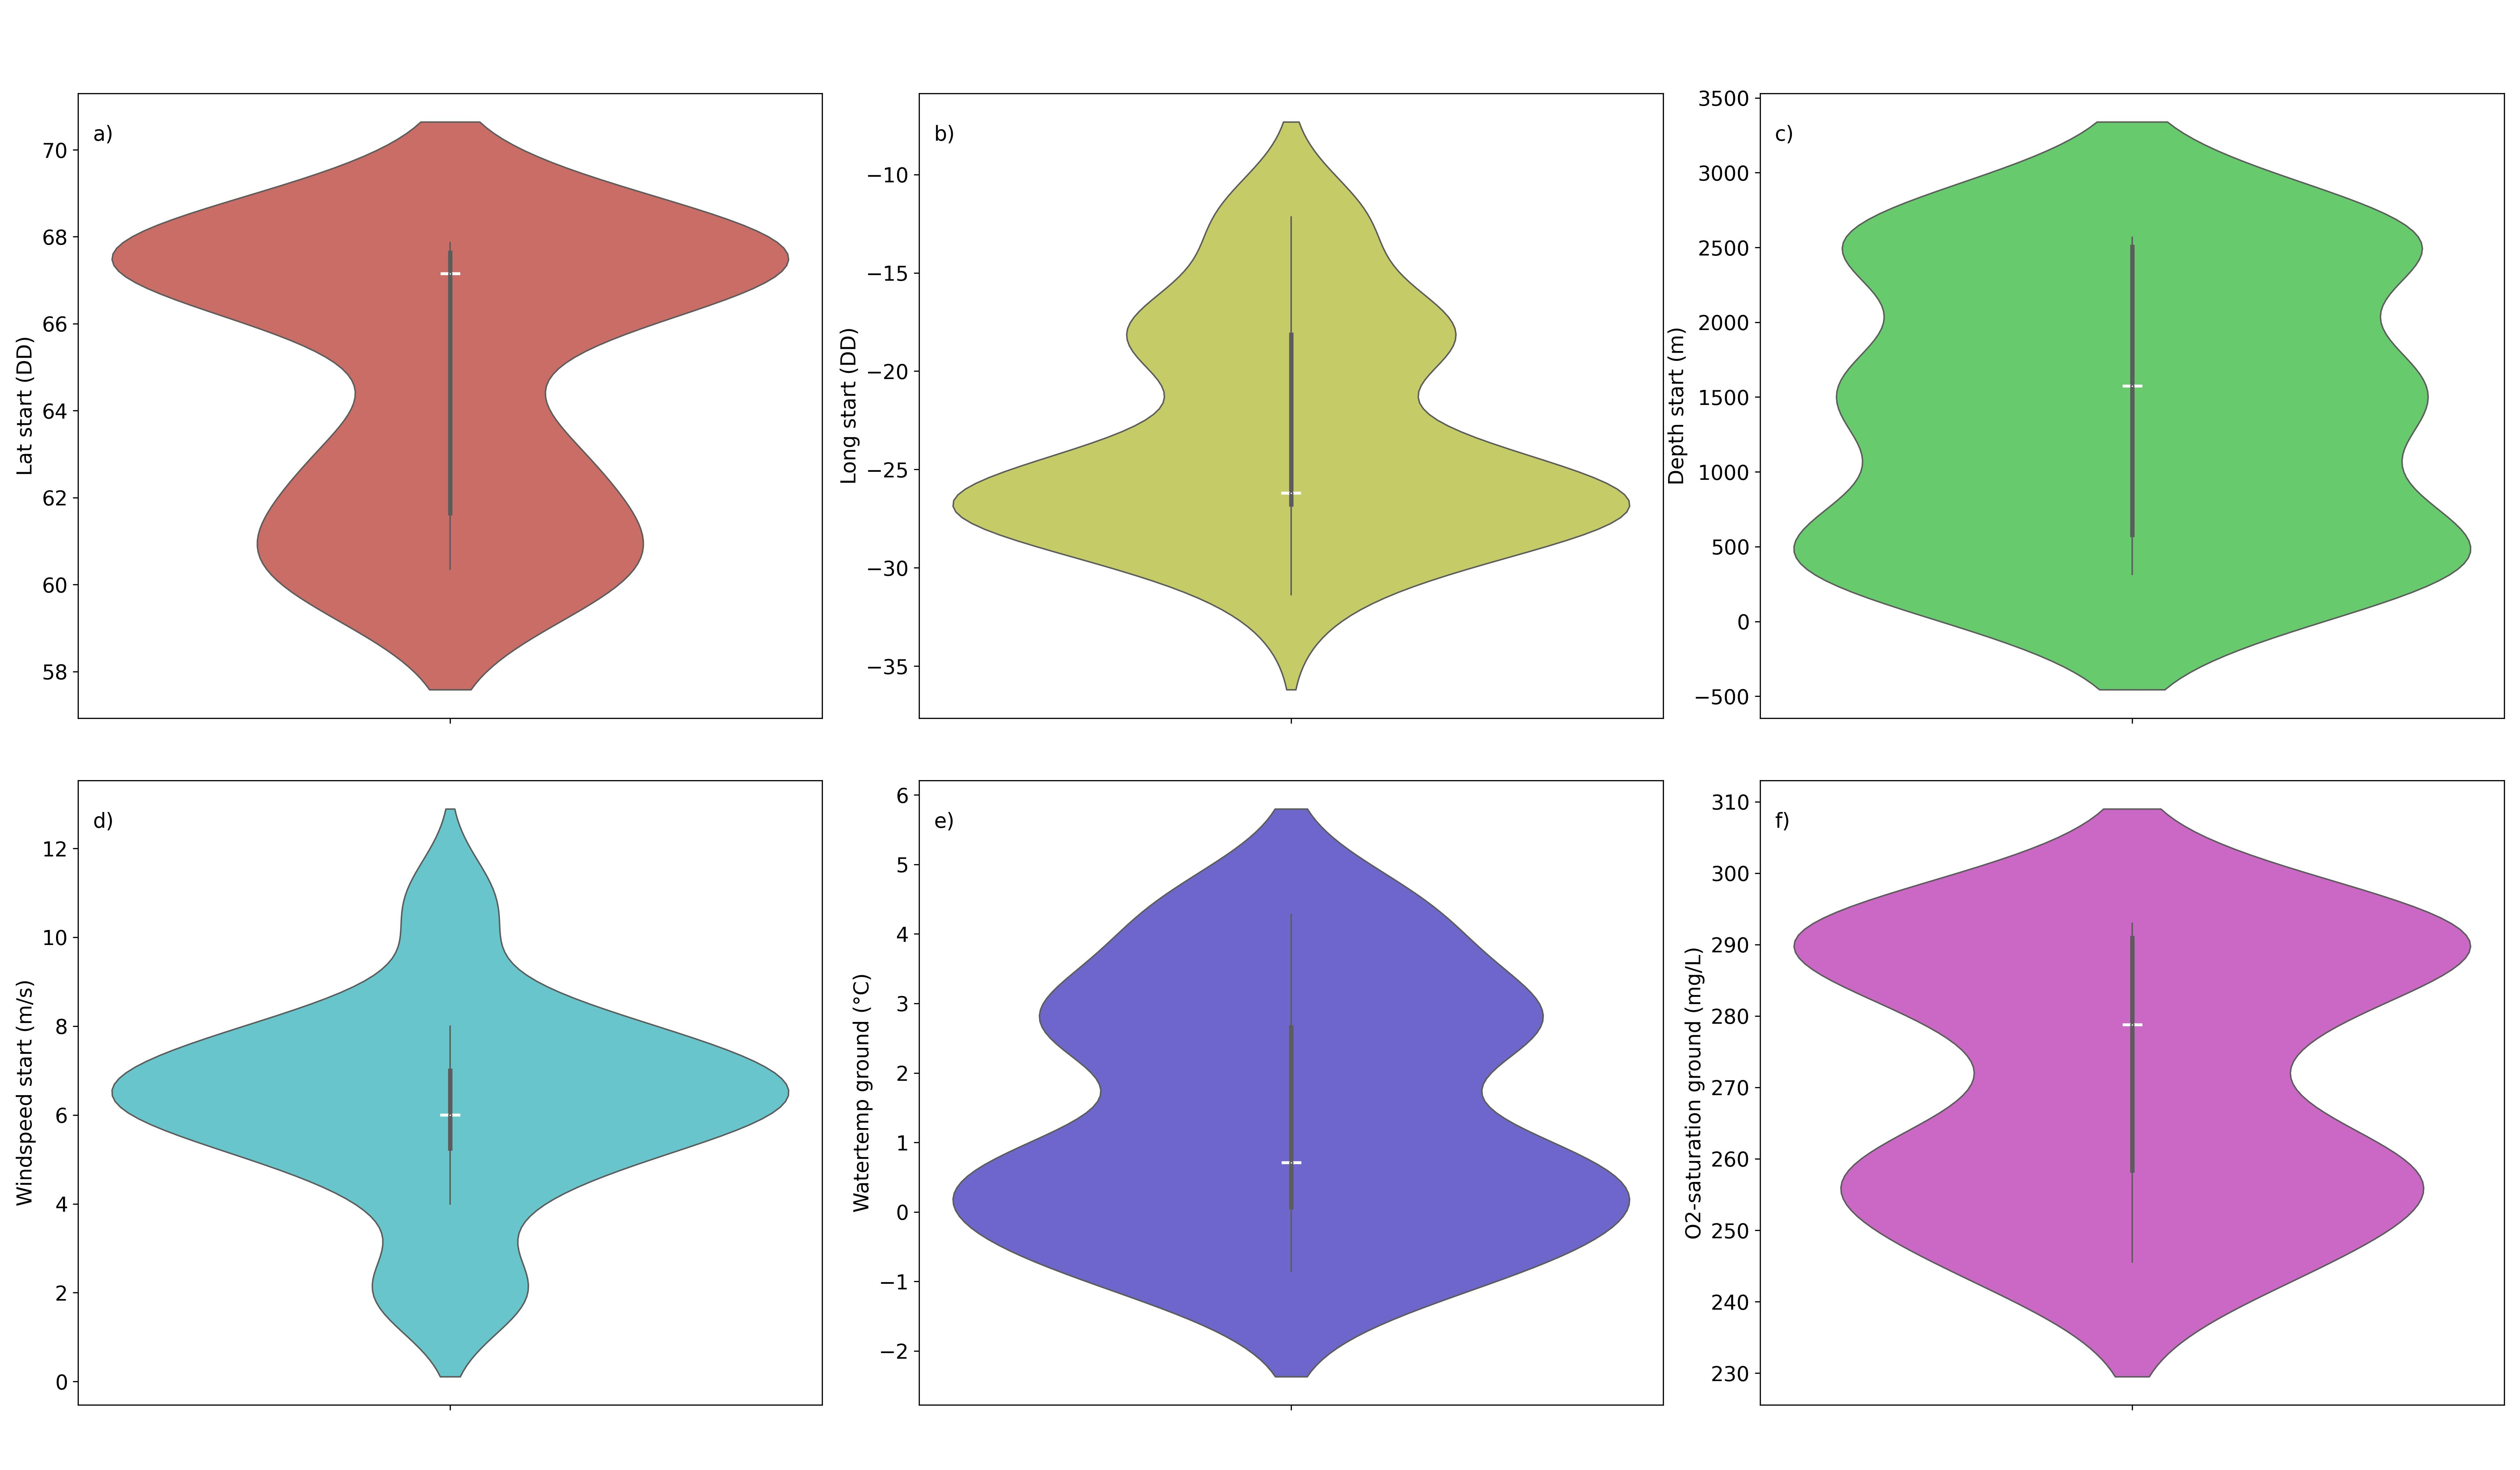
\includegraphics[width=0.7\textwidth]{figure1.jpg}
    \caption{Violin diagrams of six geographical and environmental attributes in our sample. a) Latitude (decimal) at the beginning of sampling (red); b) Longitude (decimal) at the beginning of sampling (yellow); c) Depth (m) at the start of sampling (green); d) Wind speed (m/s) at the beginning of sampling (light blue); e) Water temperature ($^\circ$C) according to the depth at which the specimens were collected (dark blue); f) Oxygen concentration (mg/L) according to the depth at which the specimens were sampled (pink). The mean, median, standard deviation (Std, Dev), 1st quartile (Q1), and 3rd quartile (Q3) of the dataset for each attribute are shown in the top right corner of each chart. \label{fig:fig1}}
\end{figure}

These diagrams are critical for designing the conditions of the habitats where the samples were collected, as high variability in the data may indicate heterogeneous habitats, while low variability indicates more homogeneous habitats. These diagrams can provide visual evidence supporting or refuting our hypothesis regarding the relationship between these environmental variables and Cumacea genetics. For example, if a correlation is found between temperature and certain genetic variations, this may support the idea that temperature influences the genetic structure of Cumacea populations. Thus, these violin plots allow to highlight rare environmental events or unique habitats that can potentially impact Cumacea genetics.

The mean, median, standard deviation, 1st and 3rd quartiles make it possible to identify general trends in the data, irregularities, or extreme values, and to capture the diversity of environmental conditions. Figure \ref{fig:fig1}a shows a latitude (decimal) range at the start of sampling of 60.357 - 67.868. The median of this distribution (67.15) is higher than the mean (64.83), indicating a skewed distribution towards lower values. This means that there are a few low values that drag the mean down. Unlike the mean, the median is less impacted by extreme values and provides an index of the central disposition of the data.  The standard deviation (3.17) shows a moderate dispersion close to the mean (64.83). The quartiles Q1 (61.64) and Q3 (67.64) reveal that the majority of data are clustered around the median (67.15). The latitude curve at the beginning of sampling has a bimodal asymmetric shape, showing two peaks, suggesting that the samples stem from two dominant latitudinal regions at the beginning of sampling. This bimodality could refer to a geographical separation of samples into two groups. This type of curve is also present for the longitude (decimal) at the beginning of the sampling as well as for the temperature ($^\circ$C) and oxygen concentration (mg/L) of the water where the samples were collected (see Figures \ref{fig:fig1}b, \ref{fig:fig1}e and \ref{fig:fig1}f). 

Figure \ref{fig:fig1}b shows a longitude (decimal) distribution at the start of sampling from -31.356 - -12.162. The median (-26.21) is lower than the mean (-23.12), suggesting an asymmetry on the side of higher values. This means that a few high values are pulling the mean upwards. The standard deviation (5.52) indicates a relatively wide range of data. Quartiles Q1 (-26.77) and Q3 (-18.14) also show high variability in the longitude data at the start of sampling.

Figure \ref{fig:fig1}c shows a depth (m) range where samples were collected of 316 - 2568. The median (1574.70) is well above the mean (1412.57), showing an asymmetrical distribution towards the lower values. The standard deviation (881.16) is quite high, indicating significant variability in sample harvesting depths at the start of sampling. Quartiles Q1 (579.10) and Q3 (2504.70) show and support, as does the standard deviation (881.16), a broad distribution of values. Significant variations in standard deviation may indicate that some environmental parameters are more variable and could possibly impact Cumacea genetics differently. The curve on this figure has a multimodal shape with three prominent peaks, suggesting that the samples were collected at various depths, reflecting the diversity of benthic habitats.

Figure \ref{fig:fig1}d shows a range of wind speeds (m/s) at the start of sampling from 2 - 11. The mean (6.26) and median (6.00) are similar, suggesting a symmetrical distribution. The standard deviation (2.16) reveals a moderate spread of the data. Quartiles Q1 (5.25) and Q3 (7.00) suggest that most wind speeds fall within a fairly narrow distribution between 5.25 and 7.00 m/s. The curve has a symmetrical shape, similar to a normal distribution, with a high concentration of data around the median (6.00), indicating relatively stable wind conditions at the beginning of sampling. 

Figure \ref{fig:fig1}e shows a temperature ($^\circ$C) distribution where samples were collected from -0.851 - 4.28. The mean (1.45) is greater than the median (0.71), demonstrating an asymmetry towards higher values. The standard deviation (1.73) is relatively high compared to the mean (1.45), indicating a wide range of data. Quartiles Q1 (0.07) and Q3 (2.66) also show an expanded dispersion of water temperature values.

Figure \ref{fig:fig1}f shows a range of oxygen concentration (mg/L) in the water where the samples were collected from 245.53 - 292.97. The median (278.77) is higher than the mean (271.88), showing an asymmetry towards the lower values. Quartiles Q1 (258.39) and Q3 (290.90) show some variability in the oxygen concentration data. This is also supported by the standard deviation (18.11).

\begin{figure}[htbp]
    \centering
    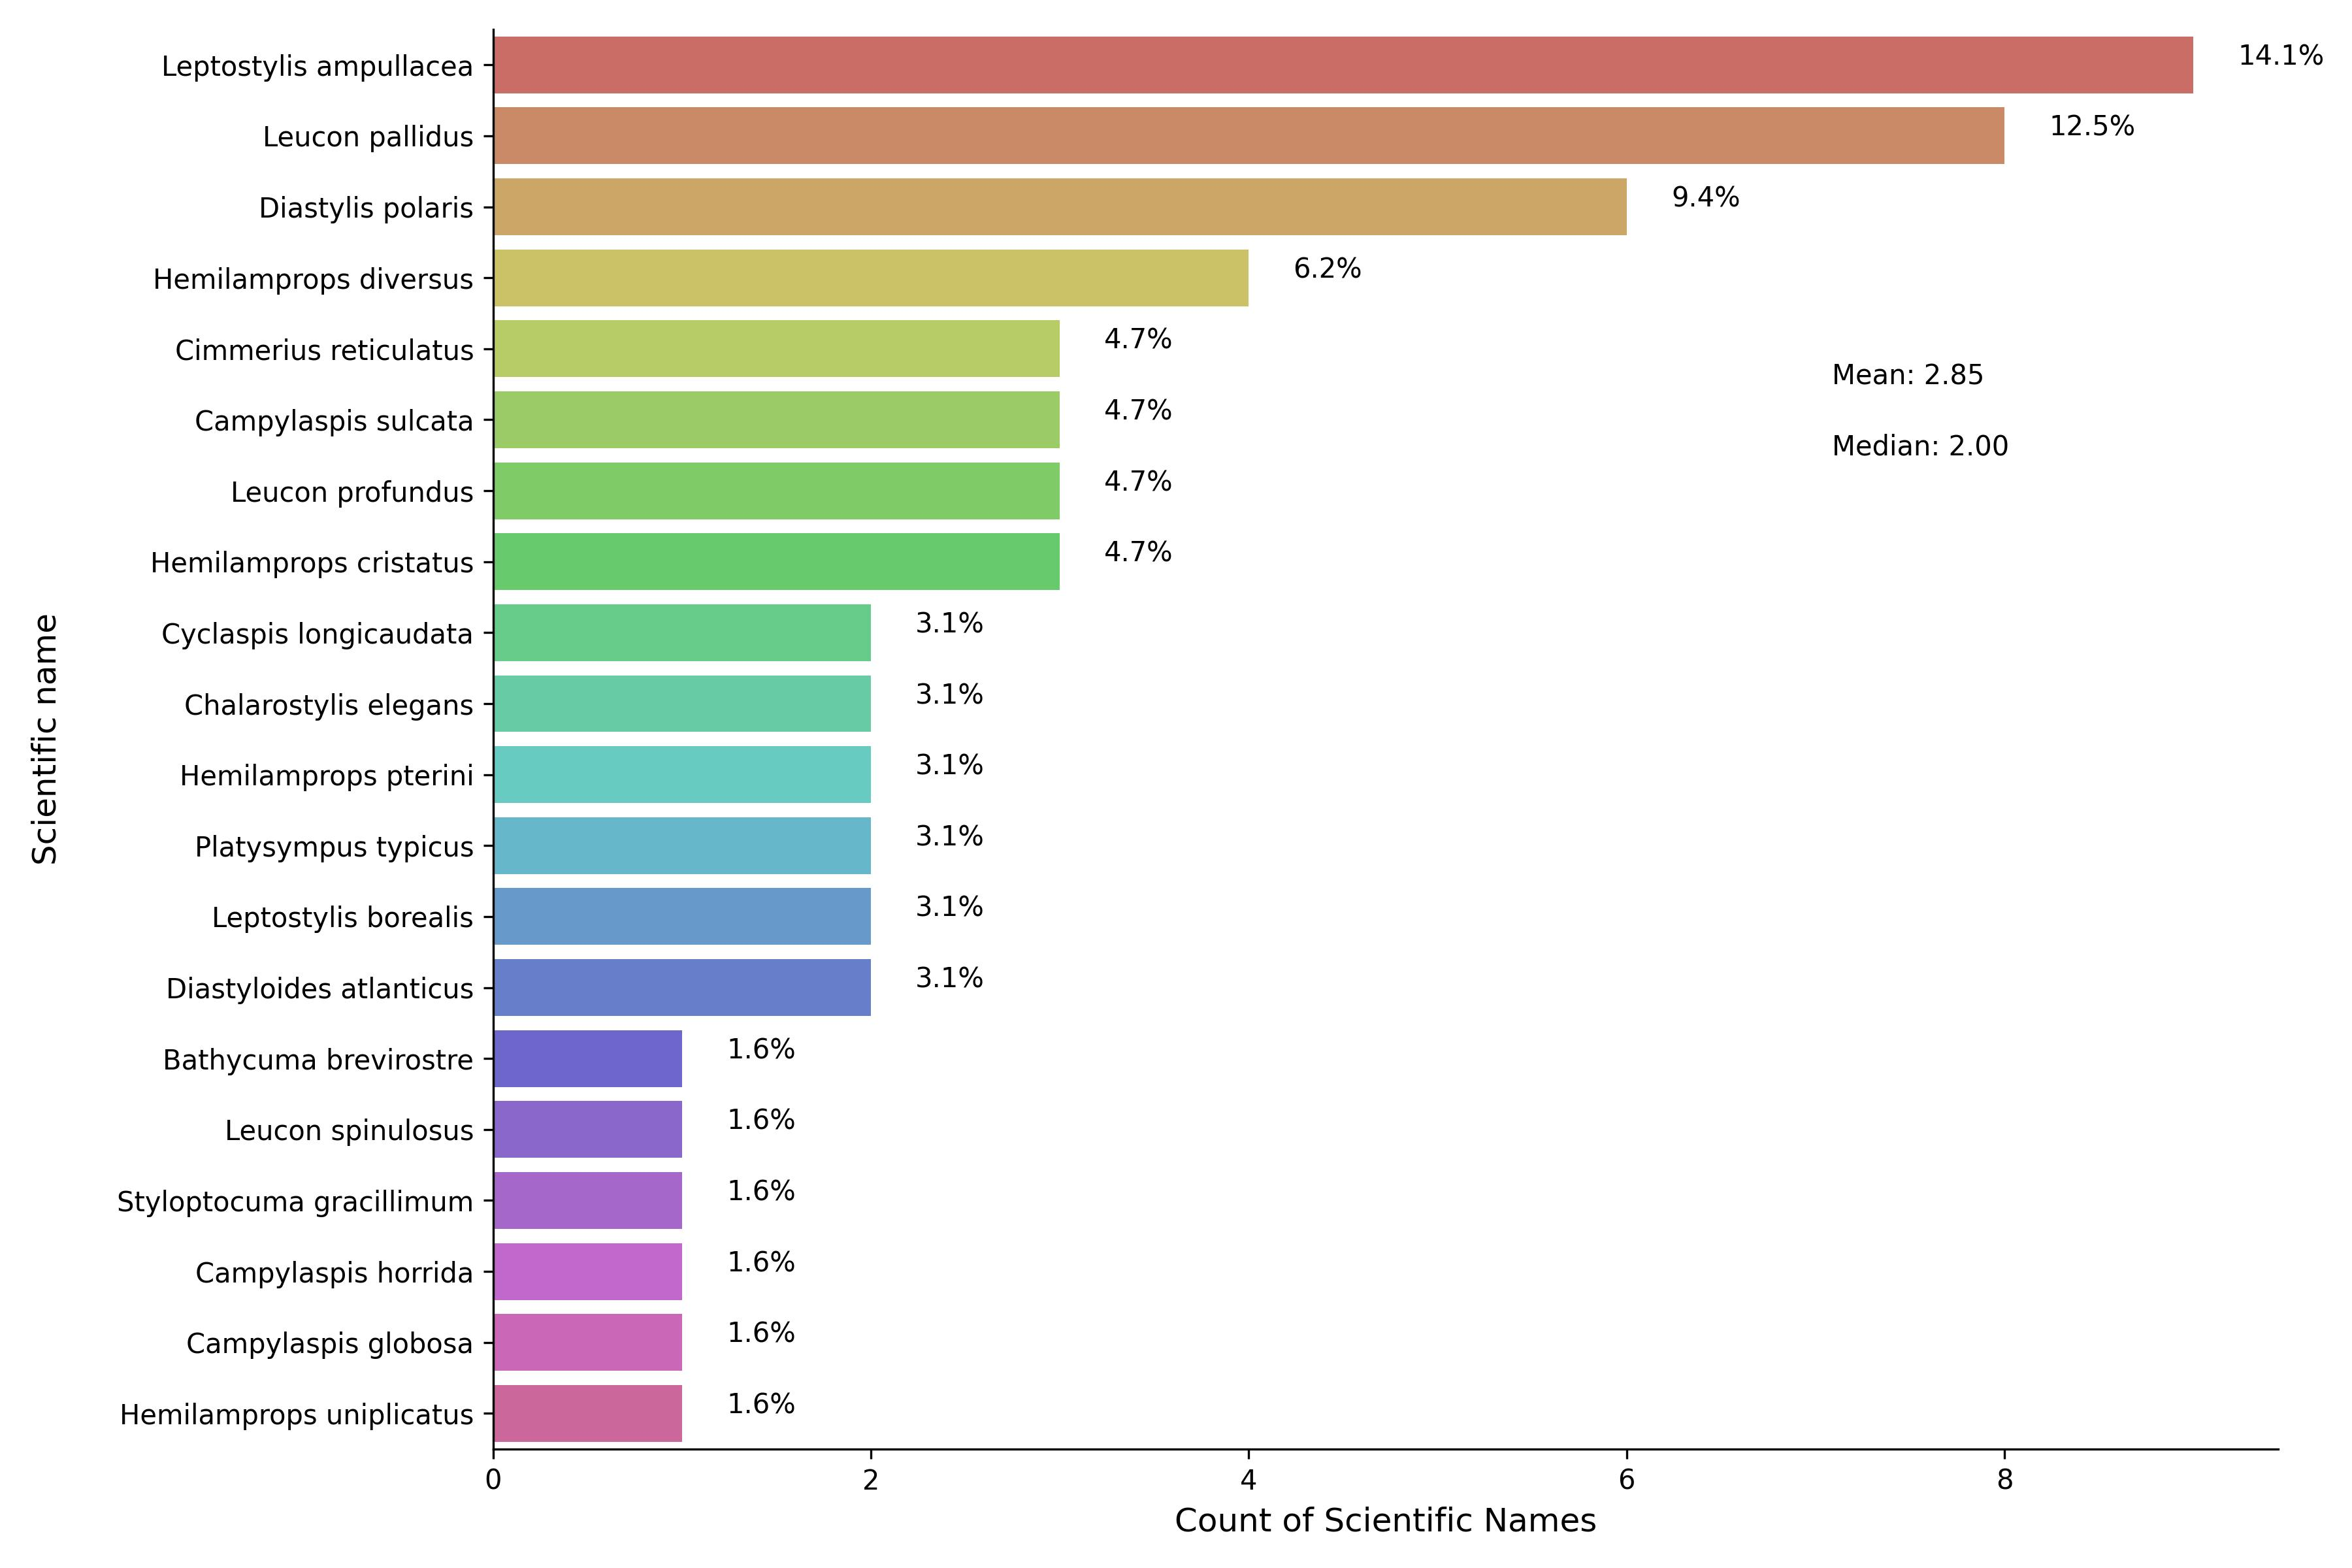
\includegraphics[width=0.7\textwidth]{figure2.jpg}
    \caption{Distribution of Cumacea Species Frequency. This histogram shows the frequency distribution of Cumacea species found in our sample. The bars represent the number of individuals for each species. The percentages displayed above the bars indicate the relative abundance (percentage) of each species within the total sample. The mean and median values of the frequency distribution are presented in the top right corner of the histogram. \label{fig:fig2}}
\end{figure}

Figure \ref{fig:fig2} presents the distribution and diversity of the different Cumacea species found in our sample and our analyses. It helps in visualizing the most represented species (\emph{Leptostylis ampullacea} and \emph{Leucon pallidus}) and the less represented species (\emph{Bathycuma brevirostre}, \emph{Leucon spinulosus}, \emph{Styloptocuma gracillimum}, \emph{Campylaspis horrida}, \emph{Campylaspis globosa}, and \emph{Hemilamprops uniplicatus}). Also, it aims to identify which species exhibit genetic diversity related to their geographical distribution, as well as to one or more local adaptations.

Comparing each species' frequency with the mean and median (see top right corner of Figure \ref{fig:fig2}) also helps to identify which species are more or less frequent. For example, as mentioned above, \emph{Leptostylis ampullacea} and \emph{Leucon pallidus}, with above-average frequencies, are dominant species. Thus, the presence of species with frequencies higher or lower than the mean and median suggests variations in sampling or particular ecological forces that advantage or disadvantage certain species. Furthermore, a median (2.00) lower than the mean (2.85) indicates that most species have relatively low frequencies, while there are a few species with higher frequencies, suggesting an asymmetrical distribution. 

\begin{figure}[htbp]
    \centering
    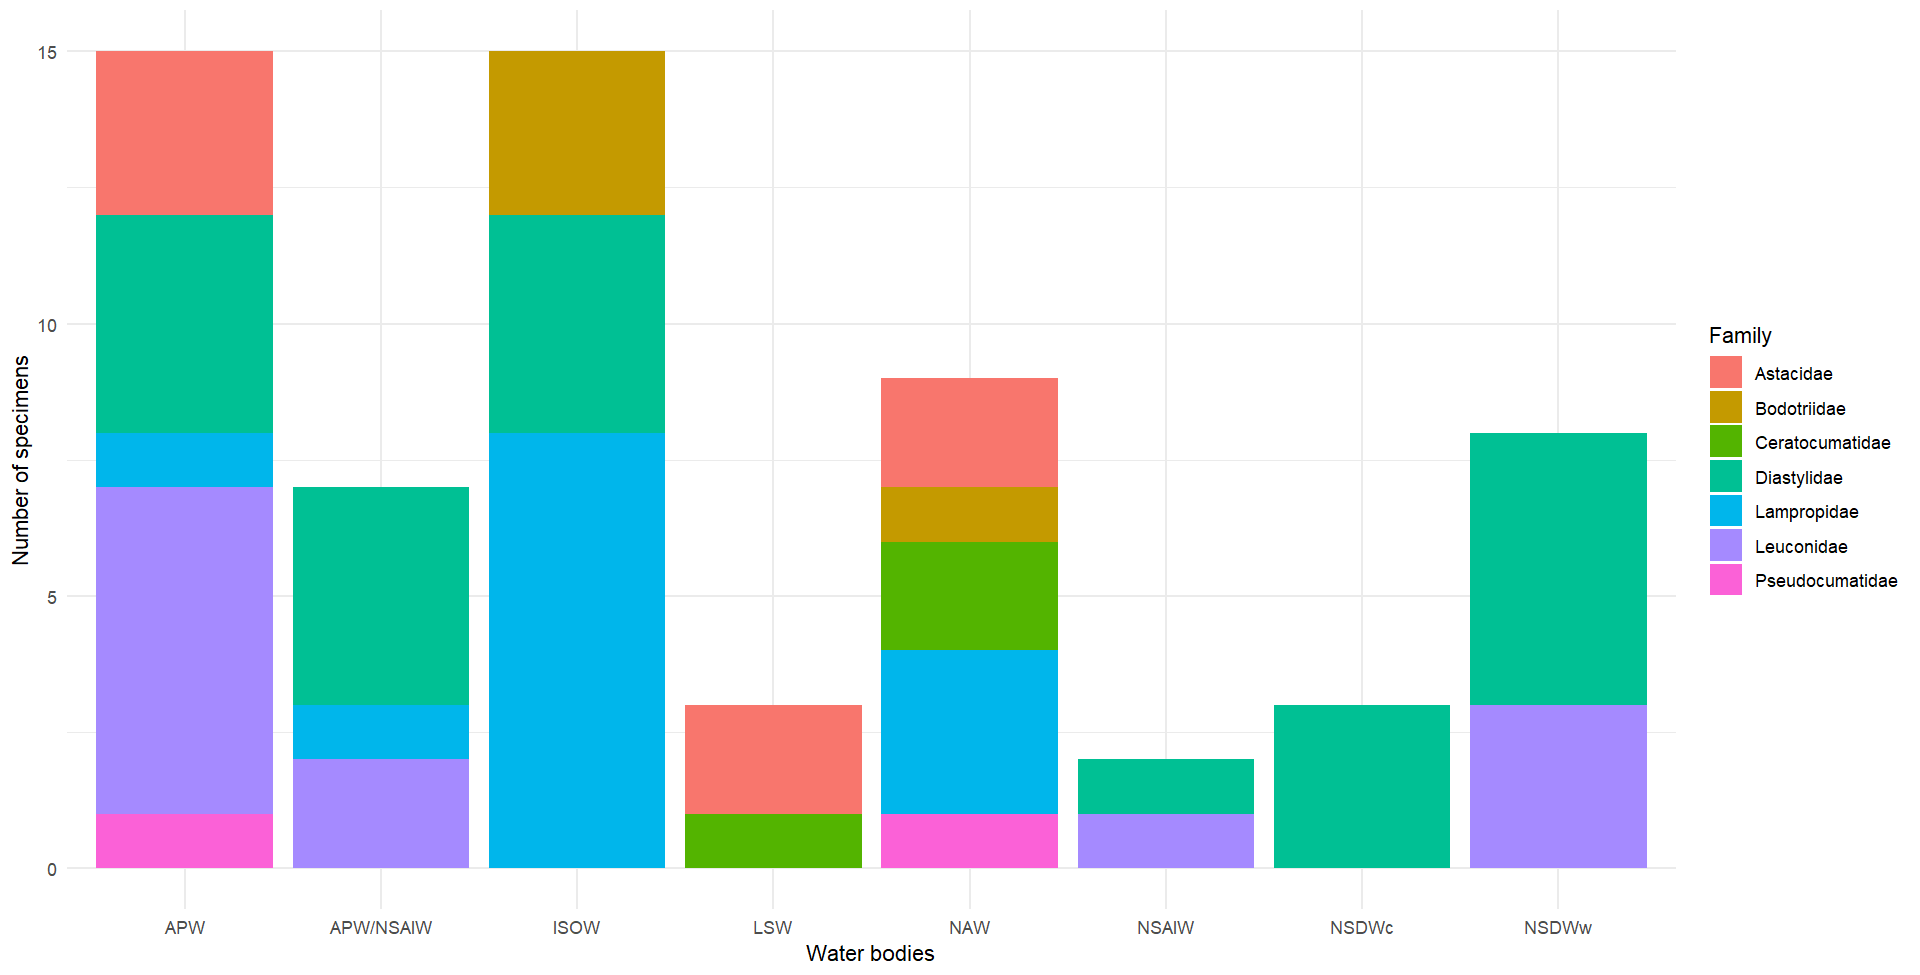
\includegraphics[width=0.7\textwidth]{figure3.png}
    \caption{Distribution of Cumacea Families by Water Body. This histogram depicts the frequency of occurrence for various Cumacea families within our samples, categorized by the water body where they were collected. Eight water body categories are represented: APW, APW/NSAIW, ISOW, LSW, NAW, NSAIW, NSDWc, and NSDWw. Seven families are represented: Astracidae (red), Bodotriidae (brown), Ceratocumatidae (green), Diastylidae (turquoise), Lampropidae (blue), Leuconidae (purple), and Pseudocumatidae (pink). \label{fig:fig3}}
\end{figure}

Figure \ref{fig:fig3} shows the distribution of samples from different Cumacea families according to the variety of water bodies where they were collected. This makes it possible to compare the diversity and potential preferences of the different families in each body of water.

APW (Arctic Polar Water) has a high family diversity, with a significant presence of the Leuconidae, Diastylidae, and Astacidae. APW/NSAIW (Arctic Polar Water/North Sub-Arctic Intermediate Water) shows a high presence of Diastylidae and Leuconidae, with a low density of Lampropidae. ISOW (Iceland Scotland Overflow Water) has a great abundance of specimens, including Lampropidae and Diastylidae. LSW (Labrador Sea Water) shows low family diversity, with a preponderance of Astacidae. NAW (North Atlantic Water), like APW (Arctic Polar Water), has a high family diversity, with a predominance of Lampropidae, Ceratocumatidae, and Astacidae. NSAIW (North Sub-Arctic Intermediate Water) shows, like LSW (Labrador Sea Water), a low family diversity, represented by the Leuconidae and the Lampropidae. NSWc and NSDWw (North Sub-Atlantic Deep Water, cold and warm), have high abundances of Diastylidae, with the presence of Leuconidae in NSDWw (warm North Sub-Atlantic Deep Water).

\begin{figure}[]
    \centering
    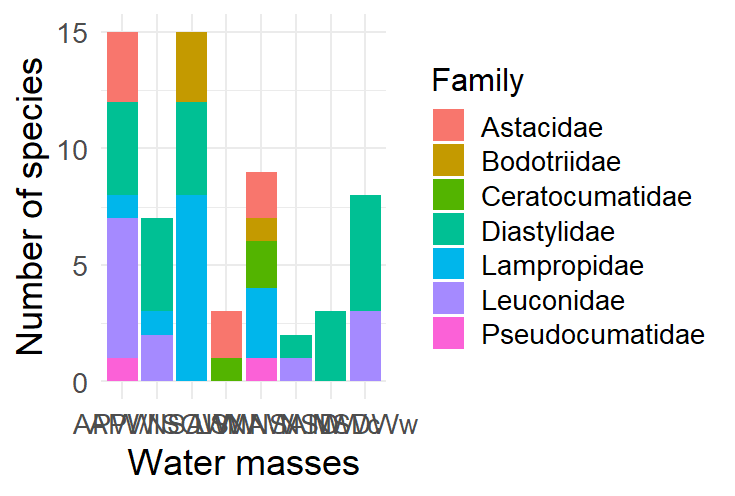
\includegraphics[width=0.7\textwidth]{figure4.png}
    \caption{Distribution of Cumacea Families by habitat. This histogram depicts the frequency of occurrence for various Cumacea families within our samples, categorized by the type of habitat where they were collected. Three habitat categories are represented: Deep sea, Shelf and Slope. Seven families are represented: Astracidae (red), Bodotriidae (brown), Ceratocumatidae (green), Diastylidae (turquoise), Lampropidae (blue), Leuconidae (purple), and Pseudocumatidae (pink).  \label{fig:fig4}}
\end{figure}

Figure \ref{fig:fig4} shows the distribution of samples from different families of Cumacea according to the type of habitat where they were collected during sampling. This makes it possible to compare the diversity of the different families in each type of housing.

Deep sea, there is a wide variety of families, dominated by the Diastylidae and the Lampropidae. Shelf presents a wide variety of family, but less than the deep sea. It is dominated by the Leuconidae. Slope, shows low family diversity, with a greater presence of Diastylidae. 

Figures \ref{fig:fig5} and \ref{fig:fig6} below show the degree of correlation between a portion of the multiple sequence alignment (i.e., windows) of our samples and two climatic parameters: wind speed at the start of sampling (m/s) and the oxygen concentration of the water where the samples were collected (mg/L). This correlation was based on four metrics: Least-Square Distance, Robinson-Fouls Distance, Normalised Robinson-Foulds Distance, and Euclidean Distance. These results were obtained using the functions leastSquare(tree1, tree2), robinsonFoulds(tree1, tree2), euclideanDist(tree1, tree2) from the \textit{aPhyloGeo} software and were organized by the main function (see \autoref{lst:main}). 

Sequence correlation raises the question of how variations in sequences (i.e., windows) respond to or vary with climatic conditions. Conserved positions (low values) could potentially suggest functionally essential regions that do not readily vary with changing climatic conditions while fluctuating positions (high values) could present specific adaptations to climatic conditions. Analyzing how sequences do or do not vary under these two different climatic conditions can highlight regions in the sequences (i.e., windows) that are sensitive or resistant to fluctuations in these two climatic parameters. In our results, we observe a similar fluctuation of the correlation with these two parameters between Figures \ref{fig:fig5} and \ref{fig:fig6}.

\begin{figure}[]
    \centering
    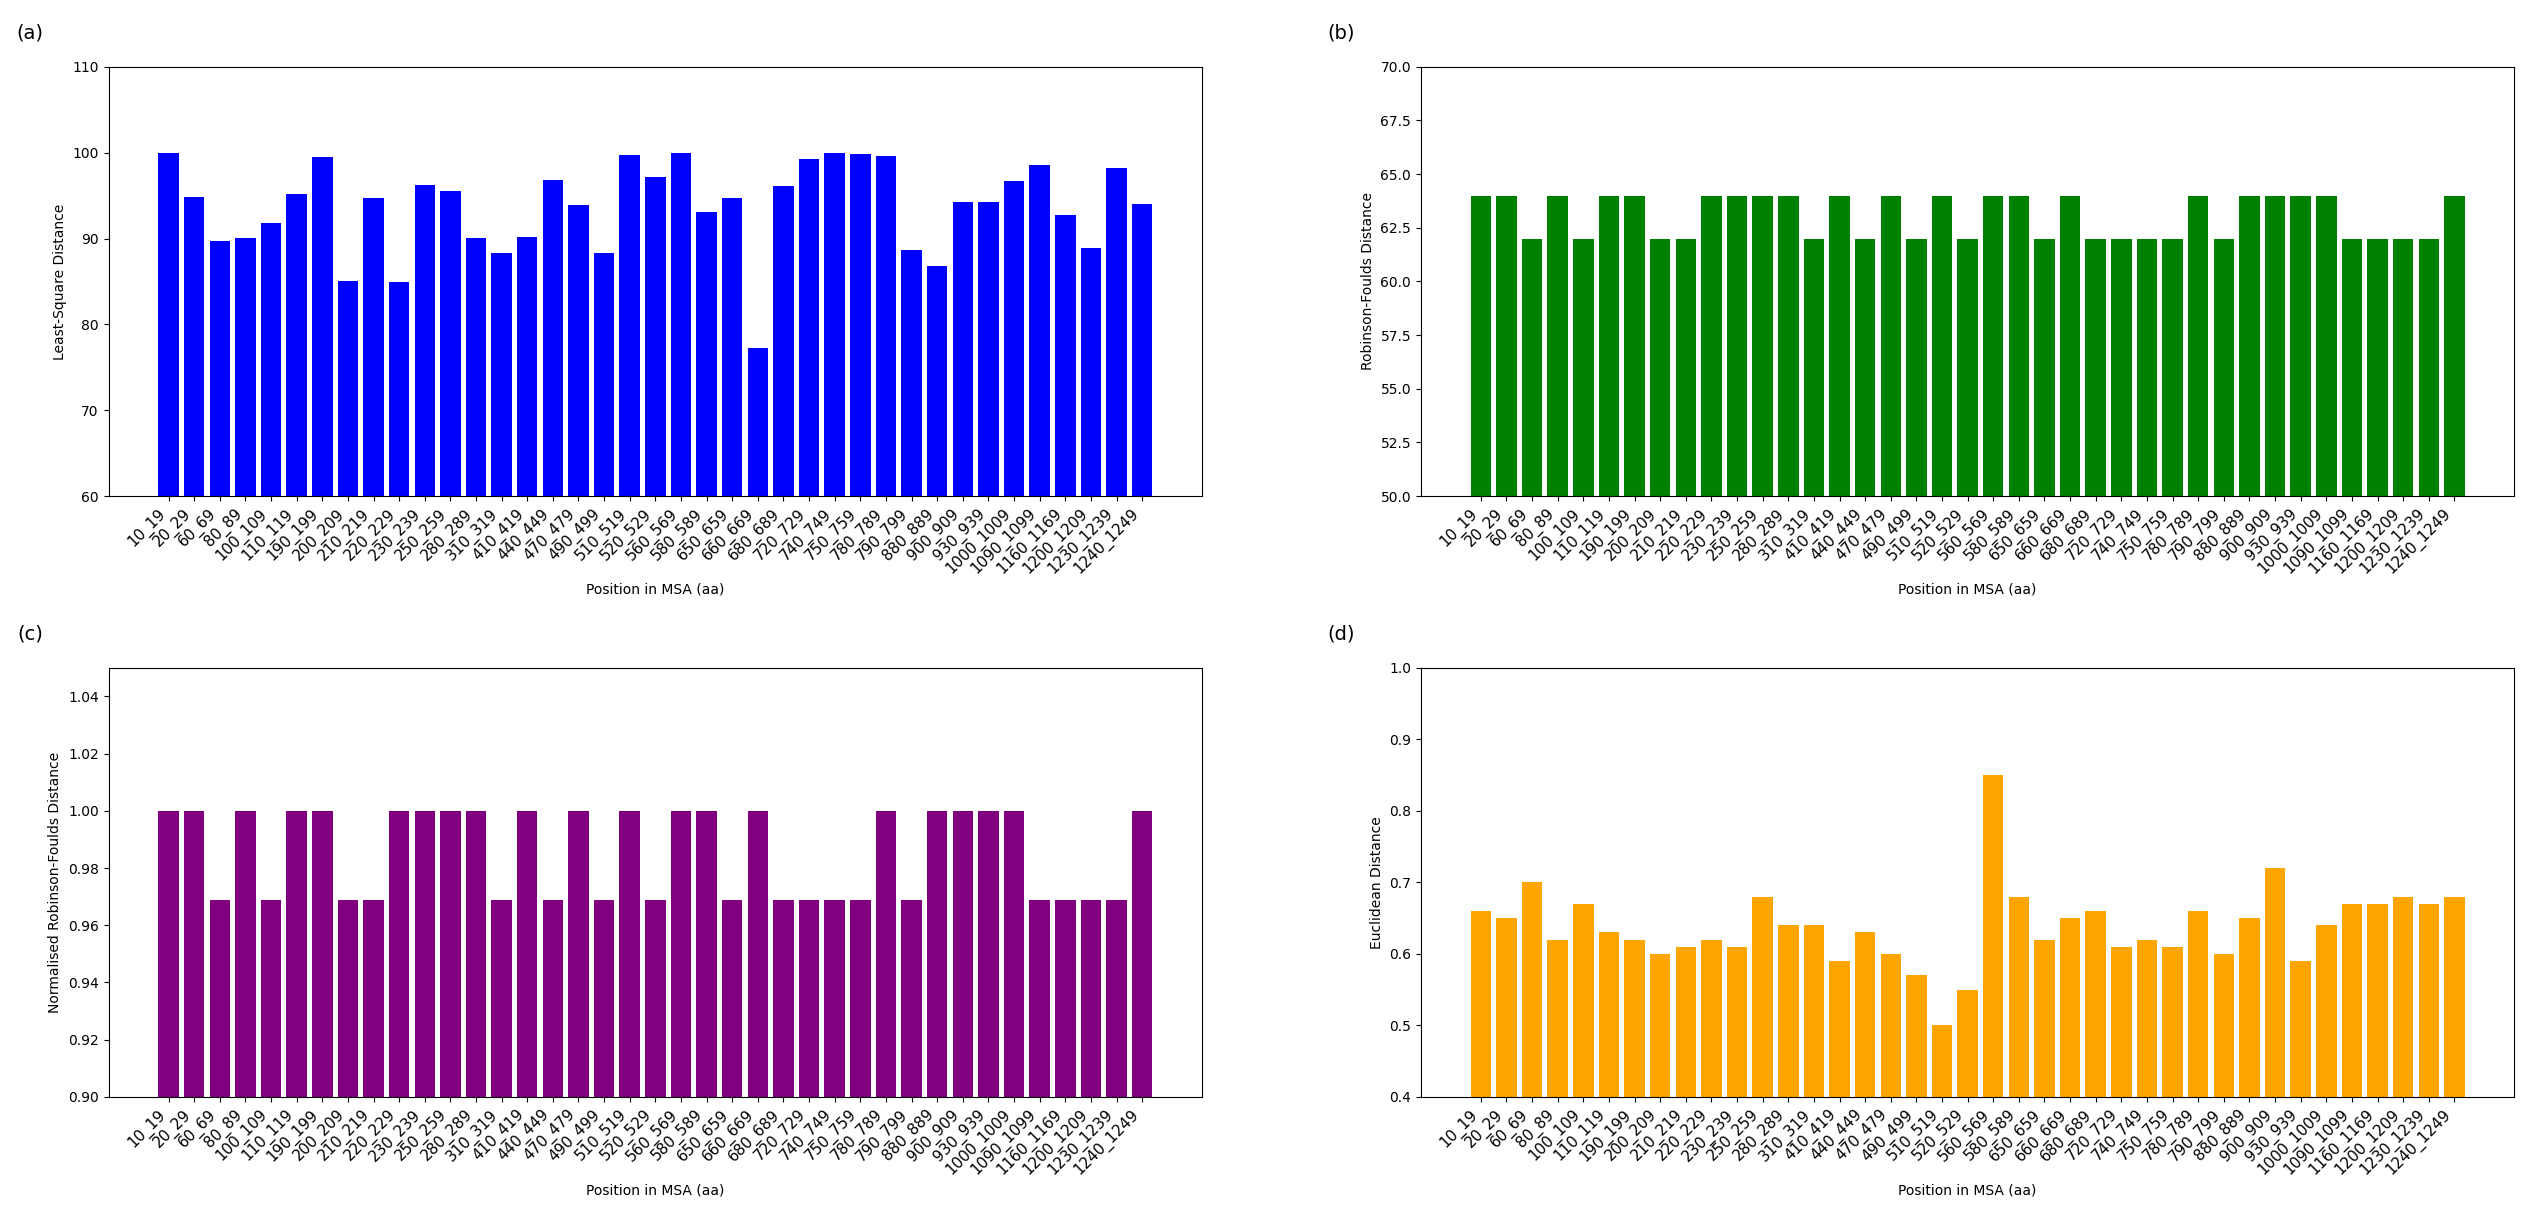
\includegraphics[width=0.7\textwidth]{figure5.png}
    \caption{Analysis of fluctuations in the four distance metrics using multiple sequence alignment (MSA): a) Least-Square distance, b) Robinson-Fouls distance, c) normalised Robinson-Fouls distance and d) Euclidean distance. These distance variations are studied to establish their correlation with fluctuations in wind speed at the start of sampling (m/s). \label{fig:fig5}}
\end{figure}

In Figure \ref{fig:fig5}a, the peaks and troughs suggest that some locations across the sample sequences are more conserved and therefore similar (smaller distance), probably indicating potential functional or structural significance, while other positions show more variability (larger distance). In contrast to Figure \ref{fig:fig5}a, the values in Figure \ref{fig:fig5}b are more concentrated on restricted values, suggesting a more uniform fluctuation. In this context, lower variation may indicate that changes in sequences do not completely affect local phylogeny. The same is true of Figure \ref{fig:fig5}c, where the normalized distances are rather homogeneous, dictating that variations in sequence positions have a fairly constant impact on the phylogenic structure of the trees. The Euclidean distance, shown in Figure \ref{fig:fig5}d, appears to be the most sensitive and disparate distance to our data. A higher Euclidean distance means a greater difference between sequences at position 520 aa to 529 aa (see Figure \ref{fig:fig5}d), suggesting that this site is more variable or evolutionarily susceptible to change. 

\begin{figure}[]
    \centering
    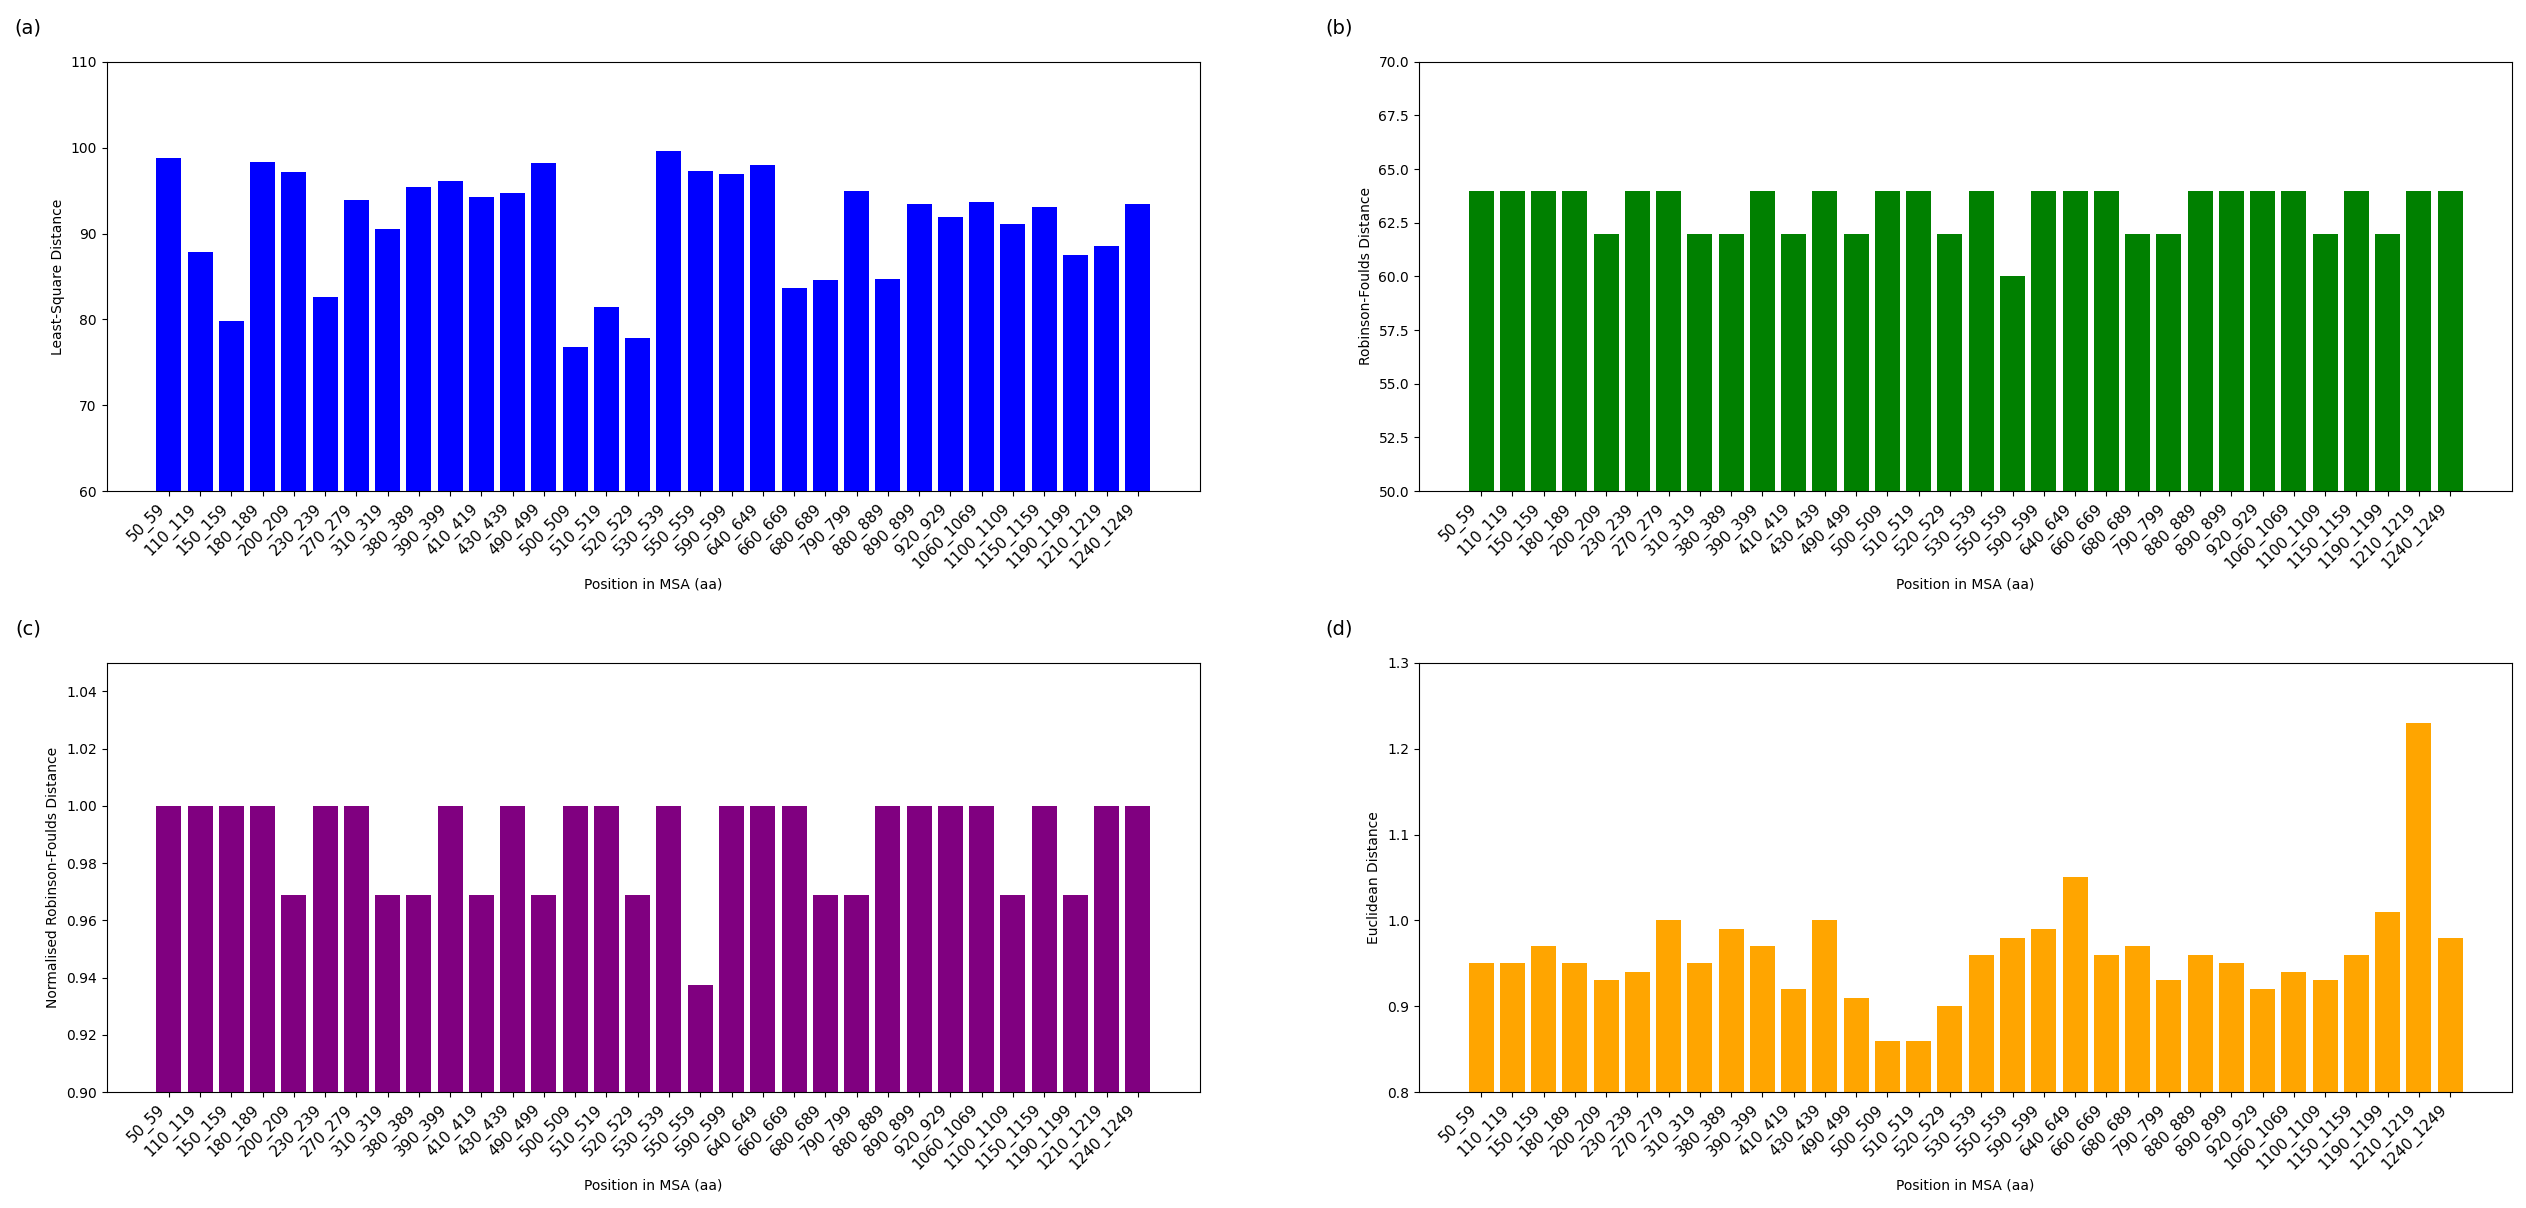
\includegraphics[width=0.7\textwidth]{figure6.png}
    \caption{Analysis of fluctuations in the four distance metrics using multiple sequence alignment (MSA): a) Least-Square distance, b) Robinson-Fouls distance, c) normalised Robinson-Fouls distance, and d) Euclidean distance. These distance variations are studied to establish their correlation with the fluctuation in oxygen concentration where the samples were collected (mg/L). \label{fig:fig6}}
\end{figure}

Figure \ref{fig:fig6}a is similar to Figure \ref{fig:fig5}a but shows more variation between different window positions. Windows with smaller mean-squared distances are more likely to be evolutionarily conserved, while windows with larger distances show greater instability. The Robinson-Foulds distances in Figure \ref{fig:fig6}b vary with a restricted range of values (50 to 70). These small variations suggest that fluctuations in sequences do not significantly alter local phylogeny. Like the figure above, Figure \ref{fig:fig6}c has a fairly homogeneous distribution. This means that variations in individual window positions exert a fairly uniform influence on the phylogenetic arrangement of trees following normalization. Like Figure \ref{fig:fig5}d, the Euclidean distance presented in Figure \ref{fig:fig6}d shows the greatest sensitivity and heterogeneity from our data. The position with the highest Euclidean distance (between 1190 aa to 1199 aa, see Figure \ref{fig:fig6}d) shows significant dissimilarity between sequences at this position, which may signify a more fluctuating or evolutionarily unstable site. 

All these results will need to be further investigated and analyzed to provide a more complete understanding of these results, and thus enable us to draw solid conclusions.

\section{Conclusion}\label{conclusion}

This study focuses on the effect of climatic variables and environmental characteristics on Cumacea (crustaceans: Peracarida) in the waters around Iceland. The main objective is to establish whether there is a correlation between the genetic information of the regions of the 16S rRNA mitochondrial gene (i.e. window) of Cumacea species and the characteristics of their habitats. Consequently, we wish to determine the environmental attribute most correlated with a specific genetic sequence, as well as the associated protein. We selected relevant attributes from the IceAGE project data, BOLD Systems, and the article by \citep{uhlir_adding_2021}. We eliminated those that were not relevant to this study, as well as those that had low variance (e.g., salinity, $S^2 = 0.02146629$) or abundant missing data (> 95\%). Using these relevant data, we incorporated, in addition to the distribution analyses of certain attributes, phylogeographic studies using the \textit{aPhyloGeo} software (see \autoref{lst:main}). The latter makes it possible to examine potential correlations between the genetics of species and their environment, thus simplifying the interpretation of the evolution of species in various environmental contexts.

The results show significant spatial variability in the Cumacea environment according to two climatic factors, such as the temperature ($^\circ$C) of the water and depth (m) (see Figures \ref{fig:fig1}e and \ref{fig:fig1}c). Excluding wind speed (m/s) at the beginning of sampling, violin diagrams present bimodal or multimodal curves, suggesting geographical and environmental separation of samples. DNA sequence analyses revealed specific genetic windows exposing high mutation rates in response to climatic variables, such as wind speed (m/s) at the start of sampling and water oxygen concentration (mg/L) (see Figures \ref{fig:fig5} and \ref{fig:fig6}). The Euclidean distances of these two parameters showed significant fluctuation across the sequences, indicating sensitive or variable sites in evolution.

The results highlight the importance of understanding the relationships between environmental attributes and genetics of benthic species such as Cumacea. This correlation can be used to explain how these organisms acclimatize to climate change as well as to anthropogenic disturbances, such as seabed mining. These notions are essential for the conservation of deep-sea ecosystems and for predicting the future impacts of environmental fluctuations on marine biodiversity. Our results can highlight conservation plans for regions sensitive to environmental and human disturbance. For example, the management of fishing and mining activities could use this knowledge to reduce their impact on benthic species. In addition, this research can guide future studies on the genetic adaptation processes of Cumacea to climatic variations.

However, further analysis is needed to examine these results in depth. Also, this study is limited by the number of samples available ($n=62$), the methods used to assess genetic and environmental properties, and the logistical burden of data collection. To consolidate these results, it would be pertinent to study other species as well as other geographic regions. In particular, interest should be shown in investigating other potentially relevant environmental attributes to better interpret the interactions between genotype and the environment.

\section{Acknowledgments}\label{acknowledgments}

The authors thank SciPy conference and reviewers for their valuable comments on this paper. This work was supported by the Natural Sciences and Engineering Research Council of Canada, the Université de Sherbrooke grant, and the Centre de recherche en écologie de l’Université de Sherbrooke (CREUS).
